\chapter{Performance}
In this chapter, we will justify some choices that we made in the code that increase efficiency.
In the process, we will show and analyze the output of some optimization tools we used in order to test the performance of this library, as well as some of the aforementioned choices.

\section{Compiler flags}
When calling the \verb|g++| complier from the \verb|Makefile|, we used the following optimization flags, which instruct the compiler to maximize the code efficiency:
\begin{verbatim}
-march=native -O3 -msse2 -funroll-loops -ftree-vectorize
\end{verbatim}
In order to test their effects, we ran the \verb|maintest_nnws.cpp| test file using 5-dimensional data, with and without the above flags, while timing both the algorithm execution and the density estimate with the help of the \verb|chrono| library.
The obtained average times (in TODO) were as follows:
\begin{center}
	\begin{tabular}{r|r|r|r}
	              	& \verb|run()| & \verb|eval_density()| & total \\ \hline
		without flags & 521762512 & 182770170 & 704532682 \\
		with flags    &  39615848 &  10353269 &  49969117 \\
		speedup       &       13x &       17x &       14x
	\end{tabular}
\end{center}
As one can see, the speedup resulting from the addition of these flags is very noticeable.





\section{Profiling analysis}
\verb|callgrind| is a command-line profiling tool that observes the running of the executable it is given as argument and records the call history among all functions that were called in it.
The output is then saved in a \verb|callgrind.out| file, which can be read with the use of the KCacheGrind GUI.
The following two commands were run, each on the C++ main test file for both the univariate case (with \verb|HierarchyNNIG<HypersFixedNNIG>|) and the multivariate case (with \verb|HierarchyNNW<HypersFixedNNW>|):
\begin{verbatim}
valgrind --tool=callgrind ./maintest_uni csv/data_uni.csv neal2 memory
valgrind --tool=callgrind ./maintest_multi csv/data_multi.csv neal2 memory
\end{verbatim}
The output of the univariate case produced the following dependence graph:
\begin{figure}[h]
	\centering
		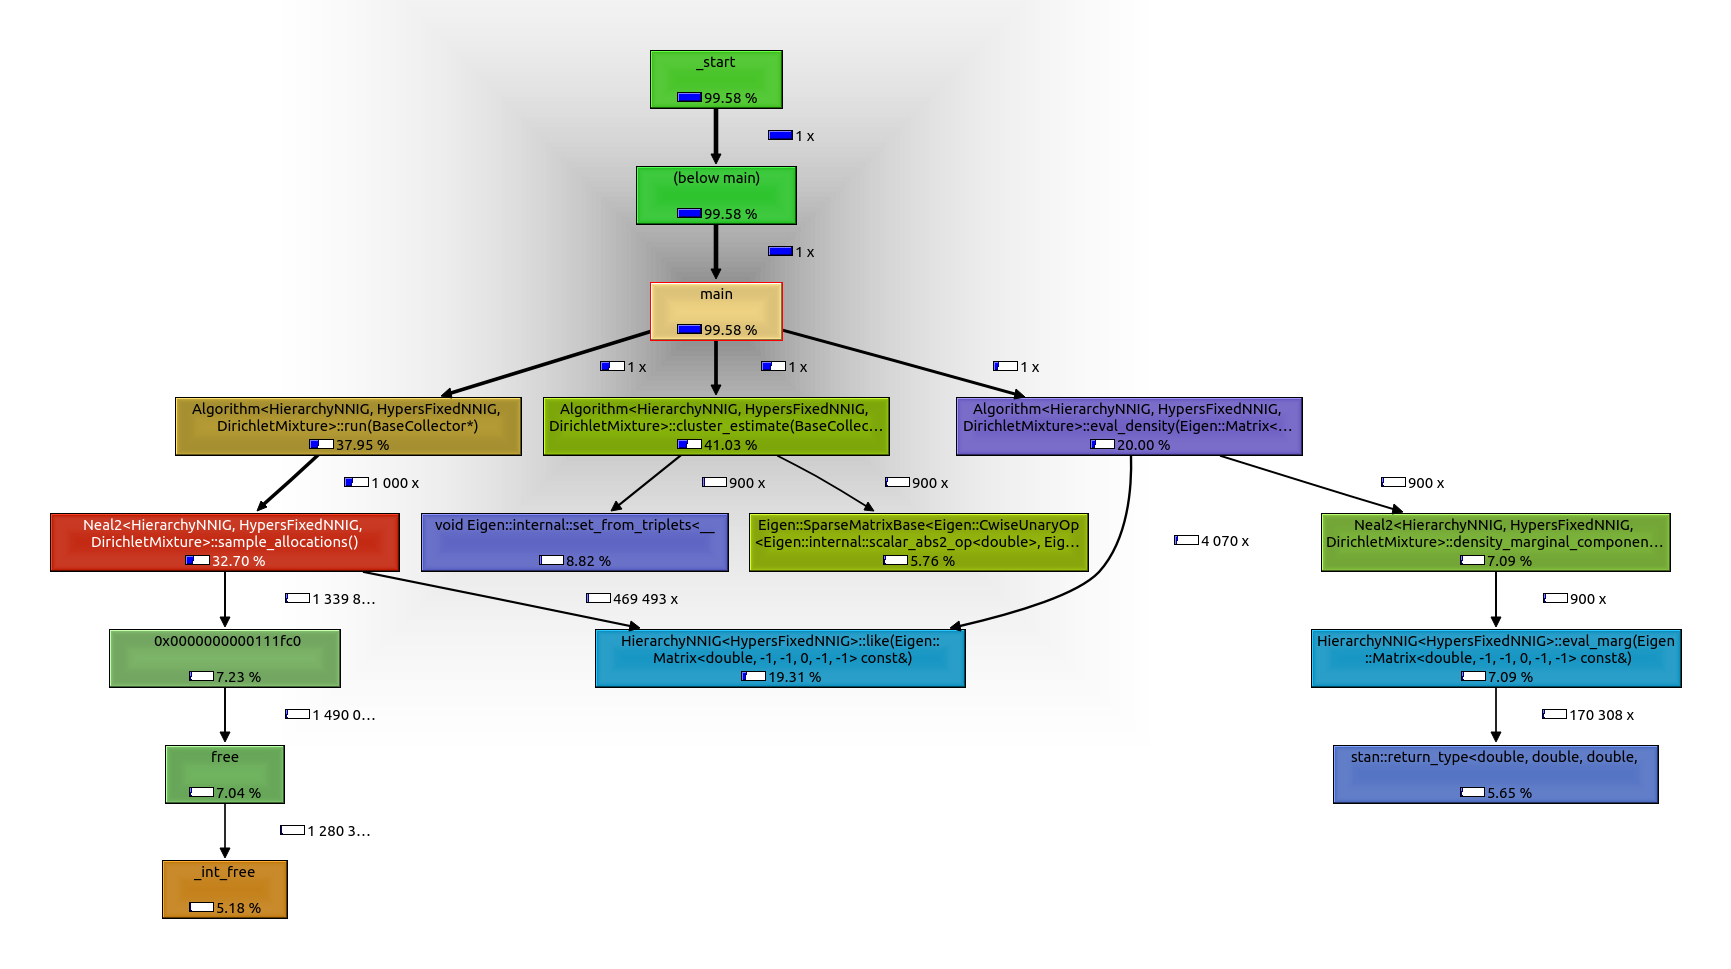
\includegraphics[scale=0.35]{etc/kcg_uni.png}
		%\captionsetup{labelformat=empty}
		%\caption{}
\end{figure}
blah blah blah TODO
\begin{figure}[h]
		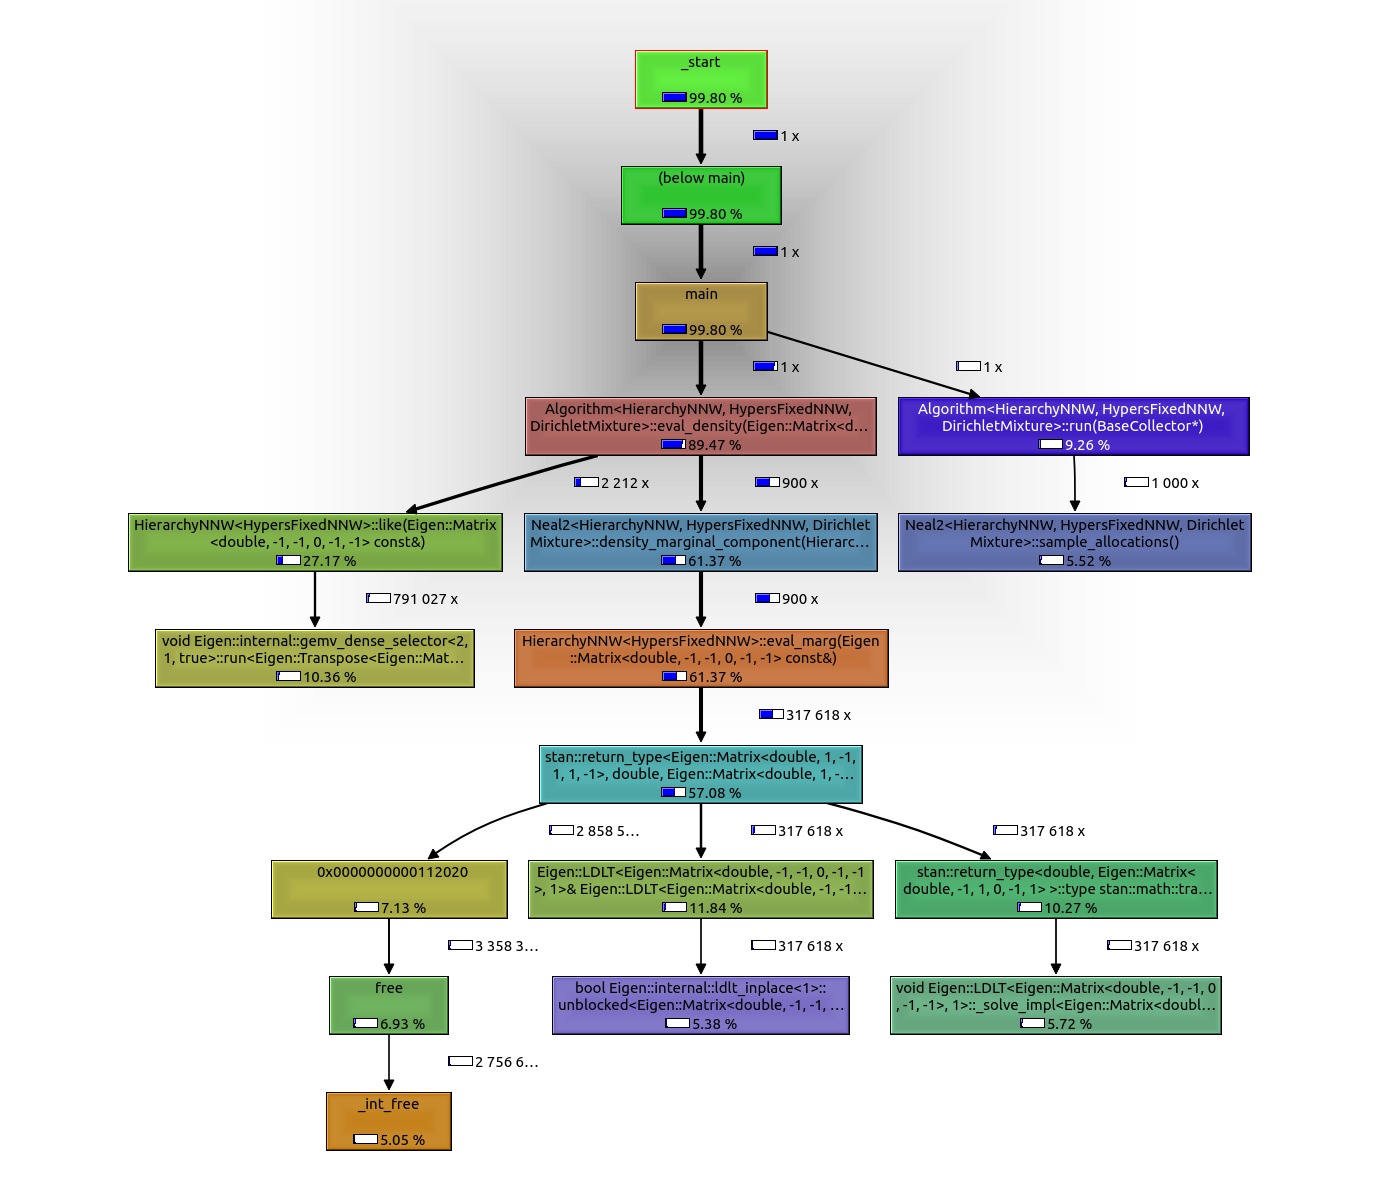
\includegraphics[scale=0.35]{etc/kcg_multi.png}
		%\captionsetup{labelformat=empty}
		%\caption{}
\end{figure}
